\documentclass[xcolor=table]{beamer}
\usepackage[utf8]{inputenc}
\usepackage[T1]{fontenc}
\usepackage[alf]{abntex2cite}
\usepackage{udesc}
\usepackage{amsfonts,amsmath,amssymb,mathtools}
\usepackage{verbatim}
\usepackage{listings}
\usepackage[ddmmyyyy]{datetime}
\usepackage{hyperref, url}
\usepackage{graphicx}
\usepackage{bussproofs}
\usepackage{multirow}
\usepackage{changepage}
\usepackage{bussproofs}	

\usepackage{svg}
\setsvg{inkscapeexe=inkscape}
\setsvg{inkscapeopt=-z -D}

\newcommand{\Ltac}{$\mathcal{L}$\unskip~tac}

\graphicspath{{Figuras/}}
\setbeamertemplate{frametitle continuation}{}

% suprimindo warnings do hyperref
\pdfstringdefDisableCommands{%
  \def\\{}%
  \def\texttt#1{<#1>}%
  \def\smallskip{}%
  \def\medskip{}%
}

\renewcommand{\figurename}{Figura}
\renewcommand{\tablename}{Tabela}
\sloppy
\title{Inferência de Tipos para CPS}

\author[Vinícios Bidin]{
    Vinícios Bidin Santos\\\smallskip
    {\scriptsize Universidade do Estado de Santa Catarina \\\smallskip
    \vspace{-2mm}
    \texttt{vinibidin@gmail.com}\\\medskip
    {Orientador: Dr.~Cristiano Damiani Vasconcellos}\\
    {Coorientador: Me. Paulo Henrique Torrens}\\
    }
}

\date{\today}

\begin{document}

    \begin{frame}
        \titlepage%
    \end{frame}

    \begin{frame}[allowframebreaks]{Sumário}
        \tableofcontents
    \end{frame}

    \section[]{Introdução}
    \begin{frame}{Introdução}
    % \begin{itemize}
    %     \item \textbf{Compilador:}
    %     \begin{enumerate}
    %         \item Tradução de código em linguagem de programação para código em linguagem de máquina
    %         \item Compilação em etapas (\textit{Front-end} e \textit{Back-end})
    %         \item Etapas ligadas por Representações Intermediárias
    %     \end{enumerate}
    % \end{itemize}
\end{frame}
    \subsection[]{Objetivos}
    \begin{frame}{Objetivo}
    \begin{itemize}
        \item Formalizar um sistema de tipos para CPS
        \item Propor e implementar em Haskell um algoritmo de inferência de tipos para CPS
        \item Validar a implementação do algoritmo por meio do teste de inferência para expressões
    \end{itemize}
\end{frame}

    \section[]{Representação Intermediária de Código}
    \begin{frame}{Representação Intermediária de Código}
    \begin{itemize}
        \item Estrutura de dados usada para manter integridade semântica e possibilitar otimizações~\cite{cooper2014}
              \begin{itemize}
                  \item[--] Classificadas de acordo com o nível de abstração
                  \item[--] Muitas vezes aplicadas em sequência
              \end{itemize}
        \item[] \begin{figure}
                  \centering
                  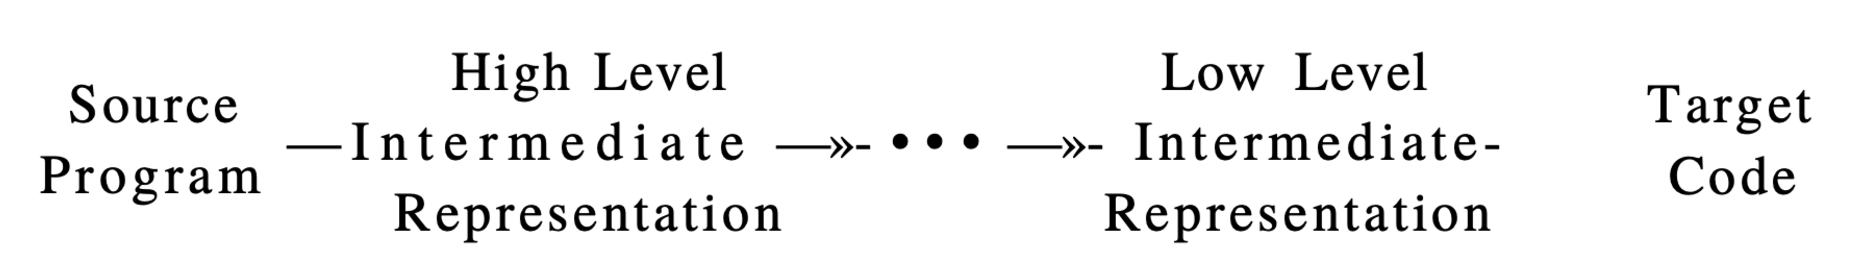
\includegraphics[width=.7\textwidth]{Imagens/abstraction-level-irs.eps}
                  \caption{Sequência de representações intermediárias}\label{fig:abstraction-level-irs}
                  \small{Fonte:~\cite{aho2008compilers}}
              \end{figure}
        \item Fluxo de controle
              \begin{itemize}
                  \item[--] Ordem das instruções
                  \item[--] Escopo
              \end{itemize}
    \end{itemize}
\end{frame}

    \subsection{Estilo de Passagem de Continuação}
    \begin{frame}{Estilo de Passagem de Continuação (CPS)}
    \begin{itemize}
        \item Técnica de transformação de código que torna o fluxo de controle explícito
              \begin{itemize}
                  \item[--] Chamadas de função passam o controle para a próxima etapa explicitamente, conhecida como continuação~\cite{appel1992compiling}
                  \item[--] Ao invés das funções retornarem o resultado da computação, é invocado uma continuação, representando o próximo passo
              \end{itemize}
        \item Toda chamada de função passa então a ser uma chamada de cauda (\textit{tail-call})
    \end{itemize}
\end{frame}

\begin{frame}{Estilo de Passagem de Continuação (CPS)}
  \textbf{Chamada de cauda:}
  \begin{itemize}
    \item Última instrução executada em uma função é uma chamada a outra função, sem que restem computações adicionais a serem feitas após essa chamada~\cite{MUCHNICK1997}
          \begin{itemize}
            \item[--] Função atual pode liberar seu quadro de ativação
          \end{itemize}
  \end{itemize}
  \textbf{Chamada não de cauda:}
  \begin{itemize}
    \item Ainda restam operações, como somas ou multiplicações, após a chamada da função
          \begin{itemize}
            \item[--] Função atual precisa manter seu quadro de ativação até que as operações sejam concluídas
          \end{itemize}
  \end{itemize}
\end{frame}

\begin{frame}{Estilo de Passagem de Continuação (CPS)}
  \begin{itemize}
    \item[] \begin{figure}
            \caption{Função fatorial em Haskell com chamada não de cauda}
            \lstinputlisting[style=haskell, label=code:factorial_non_tail_call]{Code/factorial_non_tail_call.hs}
            \small{Fonte: o autor}
          \end{figure}

    \item[] \begin{figure}
            \caption{Função fatorial em Haskell com chamada de cauda}
            \lstinputlisting[style=haskell, label=code:factorial_tail_call]{Code/factorial_tail_call.hs}
            \small{Fonte: o autor}
          \end{figure}
  \end{itemize}
\end{frame}

\begin{frame}{Estilo de Passagem de Continuação (CPS)}
  \textbf{Cálculo Lambda:}\\
  \citeonline{church1932set} define o cálculo-$\lambda$, que é representado pela seguinte gramática:

  \begin{equation}
    e ::= x \mid \lambda x. e \mid e e\nonumber
  \end{equation}

  \begin{itemize}
    \item \textbf{Variável:} identificadores no sistema
    \item \textbf{Abstração:} função que associa um identificador $x$ a um termo $e$
    \item \textbf{Aplicação:} aplicação de um termo a outro
  \end{itemize}
\end{frame}

\begin{frame}{Estilo de Passagem de Continuação (CPS)}
  Variáveis no cálculo-$\lambda$ podem ser:
  \begin{itemize}
    \item \textbf{Livres:} quando não estão associadas a uma abstração de função
          \begin{itemize}
            \item[--] $\lambda x. y$
          \end{itemize}
    \item \textbf{Ligadas:} quando estão associadas a uma abstração de função
          \begin{itemize}
            \item[--] $(\lambda x. x) y$
          \end{itemize}
    \item[]
  \end{itemize}

  Para analisar expressões:
  \begin{itemize}
    \item \textbf{$\alpha$-redução:} Renomeação de variáveis ligadas.
          \begin{align}
            \lambda x . e[x] & \rightarrow \lambda y . e[y]\nonumber
          \end{align}

    \item \textbf{$\beta$-redução:} Aplicação de função.
          \begin{align}
            (\lambda x . e_1) e_2 & \rightarrow e_1 [e_2 / x]\nonumber
          \end{align}

    \item \textbf{$\eta$-redução:} Expansão de função.
          \begin{align}
            \lambda x . (e \, x) & \rightarrow e \quad \text{se } x \text{ não ocorre livre em } e\nonumber
          \end{align}
  \end{itemize}
\end{frame}

\begin{frame}{Estilo de Passagem de Continuação (CPS)}
    \textbf{Transformação CPS:}\\
    No cálculo-$\lambda$ tradicional, o fluxo de execução é implícito
    \begin{itemize}
        \item Funções são aplicadas e os resultados são retornados
        \item $\lambda x. x + 1$
    \end{itemize}
    Já no CPS, o fluxo de execução é explícito
    \begin{itemize}
        \item Uma série de chamadas de funções passam o resultado para um argumento extra, a continuação, indicando o próximo passo da computação
        \item $\lambda x. \lambda k. k (x + 1)$
    \end{itemize}
\end{frame}

\begin{frame}{Estilo de Passagem de Continuação (CPS)}
    \textbf{Cálculo de Continuações (\textit{CPS-calculus}):}\\
    \cite{thielecke1997} define como sendo um sistema formal que trata o CPS como um modelo computacional por si só\\
    Seus termos são:
    \begin{equation}
        M ::= x\langle \vec{x} \rangle \mid M\{x\langle \vec{x} \rangle = M\}\nonumber
    \end{equation}
    \begin{itemize}
        \item \textbf{Salto (\textit{jump}):} uma chamada para a continuação $x$ com os parâmetros $\vec{x}$
        \item \textbf{Vínculo (\textit{binding}):} uma chamada onde o corpo $M$ está vinculado à continuação $x$ com os parâmetros $\vec{x}$
    \end{itemize}
\end{frame}

\begin{frame}{Estilo de Passagem de Continuação (CPS)}
    \textbf{Tradução CPS:}\\
    Converte um código escrito em estilo direto para CPS~\cite{FLANAGAN1993}
    \begin{itemize}
        \item Modificar as funções para elas não retornarem um valor, mas sim, passarem o resultado para uma continuação
    \end{itemize}
\end{frame}

\begin{frame}{Estilo de Passagem de Continuação (CPS)}
    \begin{figure}
        \caption{Função soma em Haskell em Estilo Direto}
        \lstinputlisting[style=haskell, label=code:add]{Code/add.hs}
        \small{Fonte: o autor}
    \end{figure}

    \begin{figure}
        \caption{Função soma em Haskell em CPS}
        \lstinputlisting[style=haskell, label=code:add_cps]{Code/add_cps.hs}
        \small{Fonte: o autor}
    \end{figure}
\end{frame}

\begin{frame}{Estilo de Passagem de Continuação (CPS)}
    \begin{figure}
        \caption{Função fatorial em Haskell em Estilo Direto}
        \lstinputlisting[style=haskell, label=code:factorial]{Code/fat.hs}
        \small{Fonte: o autor}
    \end{figure}

    \begin{figure}
        \caption{Função fatorial em Haskell em CPS}
        \lstinputlisting[style=haskell, label=code:factorial_cps]{Code/fat_cps.hs}
        \small{Fonte: o autor}
    \end{figure}
\end{frame}

% \begin{frame}{Estilo de Passagem de Continuação (CPS)}
%     \textbf{Tranformação dos Tipos:}\\
%     Função em Estilo direto
%     \begin{itemize}
%         \item $A \rightarrow B$
%     \end{itemize}
%     Função em CPS
%     \begin{itemize}
%         \item $A \rightarrow (B \rightarrow \perp) \rightarrow \perp$
%     \end{itemize}

%     % Na função de soma, definida na Figura~\ref{code:add}, a função tem tipo $Int \rightarrow Int \rightarrow Int$, ou seja, ela recebe dois inteiros e retorna um inteiro.
%     % Já a função de soma em CPS, definido na Figura~\ref{code:add_cps}, possui o tipo $Int \rightarrow Int \rightarrow (Int \rightarrow r) \rightarrow r$. Isso significa que a função recebe dois inteiros e uma continuação, que é uma função de tipo $Int \rightarrow r$, onde \texttt{r} pode ser qualquer tipo, e retorna esse mesmo tipo \texttt{r}.

%     % Essa transformação de tipo reflete a diferença fundamental entre o estilo direto e o CPS\@: em vez de retornar um valor diretamente, a função em CPS recebe uma continuação que especifica o próximo passo da computação.
%     % O mesmo padrão pode ser observado nas funções para o cálculo do fatorial nas Figuras~\ref{code:factorial} e~\ref{code:factorial_cps}.
%     % No estilo direto, a função \texttt{factorial} tem o tipo $Int \rightarrow Int$, enquanto na versão CPS, a função \texttt{factorialCps} tem o tipo $Int \rightarrow (Int \rightarrow r) \rightarrow r$.

%     % Essa correspondência entre os tipos não é uma coincidência.
%     % Como discutido por~\cite{TORRENS2019}, uma função em estilo direto com tipo $A \rightarrow B$ pode ser transformada em uma função em CPS com o tipo $A \rightarrow (B \rightarrow \perp) \rightarrow \perp$.
%     % Aqui, $\perp$ representa o tipo dos valores que nunca retornam, uma característica associada ao estilo de passagem de continuações, onde as funções são compostas de forma a encadear continuações até que a execução termine de maneira explícita.
% \end{frame}


    \section[]{Teoria de Tipos}
    \section{Teoria de Tipos}\label{sec:type-theory}

A Teoria de Tipos, conforme apresentada por~\cite{COQUAND2022}, foi introduzida por Russell em 1908 ao encontrar um paradoxo na Teoria de Conjuntos, conhecido atualmente como o Paradoxo de Russell:

\begin{equation}\label{eq:russell-paradox}
  \text{Seja } R = \{ x \mid x \notin x \}, \text{ então } R \in R \iff R \notin R
\end{equation}

Ou seja, considere $R$ como o conjunto dos conjuntos que não contêm a si mesmos.
A contradição surge ao observar que, se o conjunto $R$ contém a si mesmo, isso implica que $R$ não contém a si mesmo, e vice-versa.

Outra maneira de descrever esse paradoxo é através do Paradoxo do Barbeiro: imagine uma cidade com apenas um barbeiro, onde ele somente barbeia aqueles que não se barbeiam.
O paradoxo surge quando perguntamos: ``Quem barbeia o barbeiro?''
Ele não pode fazer sua própria barba, pois barbeia apenas aqueles que não fazem a própria barba.
No entanto, se ele não faz sua própria barba, então pertence ao grupo daqueles que devem ser barbeados pelo barbeiro, logo, ele deveria barbear-se.
Essa situação gera uma contradição semelhante ao Paradoxo de Russell.

Atualmente, a principal aplicação da Teoria de Tipos está na formalização de sistemas de tipos para linguagens de programação.
Um sistema de tipos garante a ausência de certos comportamentos dos programas classificando os valores computados em cada uma de suas sentenças~\cite{PIERCE2002}.
Além disso, atribuir e verificar tipos para cada construção presente nos programas têm várias utilidades, como fornecer informações para auxiliar na modularização de programas, otimização de código executada pelo compilador e também pode ser usada como documentação do código.
Sistemas de tipos também são usados na construção de assistentes de provas, por exemplo, o Coq utiliza o Cálculo de Construções~\cite{COQUAND1998}.
Linguagens como Idris e Agda, que são funcionalmente dependentes, também permitem a verificação de provas formais.

No contexto das linguagens de programação, podemos distinguir três categorias principais de tipos: tipos simples, tipos polimórficos e tipos dependentes~\cite{PIERCE2002}.
Tipos simples atribuem um tipo fixo a cada termo, enquanto tipos polimórficos introduzem a noção de generalidade, permitindo que funções possam ser aplicadas a argumentos de diferentes tipos sem a necessidade de serem redefinidas para cada um.
Já os tipos dependentes permitem que tipos dependam de valores.

Um exemplo de tipo simples é uma função que opera sobre números inteiros.
Esta função recebe um número inteiro e retorna outro número inteiro.
Seu tipo, portanto, é representado como $Int \rightarrow Int$, indicando que tanto a entrada quanto a saída são do tipo inteiro.

Um exemplo de polimorfismo é a função identidade, que recebe um elemento de qualquer tipo e retorna o mesmo elemento.
Seu tipo é expresso como $a \rightarrow a$, onde $a$ pode ser qualquer tipo.
Este tipo polimórfico indica que a função identidade pode ser usada com diferentes tipos de dados sem precisar ser modificada.

Em linguagens com suporte a tipos dependentes, um exemplo seria o de um vetor cujo comprimento (número de elementos) faz parte de seu tipo.
Nesse caso, uma função de concatenação de vetores deve garantir que somente vetores com tipos compatíveis em relação ao comprimento possam ser concatenados.
O tipo da função de concatenação seria algo como\footnote{A notação exata pode variar entre diferentes linguagens de programação que suportam tipos dependentes. A estrutura apresentada serve apenas como uma ilustração conceitual do comportamento esperado.} $Vector(n) \rightarrow Vector(m) \rightarrow Vector(n+m)$, onde $n$ e $m$ são valores que representam os comprimentos dos vetores e fazem parte da definição de tipo.

No contexto do polimorfismo,~\citeonline{PIERCE2002} define duas principais variedades: o polimorfismo paramétrico, que permite que uma única definição de função opere de maneira genérica, e o polimorfismo com sobrecarga, que permite que uma função tenha diferentes comportamentos dependendo do tipo dos argumentos.
No polimorfismo paramétrico, como no caso da função identidade, todas as instâncias de uma função genérica compartilham o mesmo comportamento, independentemente dos tipos específicos com os quais são instanciadas.
Já no polimorfismo com sobrecarga, o comportamento da função pode variar conforme o tipo dos dados, como acontece com sobrecarga de operadores. Uma função sobrecarregada pode ter múltiplas implementações, com a seleção adequada dependendo dos tipos dos argumentos.

O polimorfismo desempenha um papel crucial na inferência de tipos.
Em linguagens com suporte a inferência de tipos, como Haskell, o sistema de tipos é capaz de deduzir tanto tipos específicos quanto tipos genéricos, sempre que possível, para permitir polimorfismo~\cite{PIERCE2002}.
O polimorfismo refere-se à capacidade de uma função ou expressão operar sobre diferentes tipos de dados de forma genérica.
Um exemplo clássico é a função identidade, $\lambda x.x$, que pode ser tipada como $\forall \alpha. \alpha \to \alpha$, indicando que a função aceita um valor de qualquer tipo $\alpha$ e retorna um valor do mesmo tipo.
Esse tipo é conhecido como polimorfismo universal~\cite{PIERCE2002}.

Já a função de soma apresentada na Figura~\ref{code:add} demonstra outro tipo de polimorfismo.
Como possui tipagem explícita $Int \rightarrow Int \rightarrow Int$, apenas valores do tipo inteiro podem ser somados.
No entanto, essa mesma função pode ser generalizada para permitir a soma de quaisquer números, desde que sejam do mesmo tipo, utilizando restrições de classe de tipos.

Em Haskell, uma classe de tipos é um conjunto de tipos que compartilham um conjunto comum de operações, e as classes de tipos são a maneira pela qual a linguagem lida com sobrecarga.
Por exemplo, a função \texttt{sumList}, que calcula a soma dos elementos de uma lista, pode ser definida com uma restrição de classe, na Figura~\ref{code:sum_list}.

\begin{figure}
  \caption{Função somatório de elementos de lista em Haskell}
  \small{Fonte: o autor}
  \lstinputlisting[style=haskell, label=code:sum_list]{Code/sum_list.hs}
\end{figure}

Aqui, a restrição \texttt{Num a} indica que \texttt{sumList} pode operar sobre listas de qualquer tipo \texttt{a}, desde que \texttt{a} pertença à classe \texttt{Num}, que define os tipos numéricos em Haskell.
Dessa forma, a função permite a soma de inteiros, valores \texttt{Float}, \texttt{Double} e outros tipos numéricos.

O polimorfismo restrito (ou polimorfismo de sobrecarga) é o que permite essa generalização~\cite{PIERCE2002}, pois a função é capaz de operar sobre múltiplos tipos, mas dentro de uma classe específica de tipos, garantindo flexibilidade e segurança no sistema de tipos.

O Cálculo Lambda Simplesmente Tipado é uma das primeiras e mais simples variantes do Cálculo Lambda que incorpora tipos em sua estrutura~\cite{CHURCH1940}.
Enquanto o cálculo lambda original não faz distinção entre diferentes tipos de dados, no Cálculo Lambda Simplesmente Tipado, os termos são anotados com tipos.
Cada função recebe e retorna valores de tipos específicos, o que permite prevenir uma série de erros comuns em programas, como a aplicação de funções a argumentos incorretos.

Além disso, o sistema de tipos serve como uma ferramenta de verificação durante a compilação de programas, assegurando que erros de tipo sejam detectados antes da execução.
Dessa forma, ele não apenas facilita a criação de software mais robusto, mas também oferece uma base formal para o estudo de linguagens de programação~\cite{PIERCE2002}.

A sintaxe básica do Cálculo Lambda Simplesmente Tipado inclui:

\begin{itemize}
  \item Variáveis: $x, y, z, \ldots$
  \item Tipos: $T ::= \mathbf{Int} \mid \mathbf{Bool} \mid T \to T$
  \item Termos: $\lambda x:T. \tau \mid \tau_1 \tau_2 \mid x$
\end{itemize}

No Cálculo Lambda Simplesmente Tipado, cada variável possui um tipo atribuído e os termos são construídos com base nesses tipos.
Por exemplo, a abstração de função $\lambda x:T. \tau$ define uma função onde a variável $x$ é de tipo $T$ e o corpo da função, $\tau$, é um termo.
A aplicação de função $\tau_1 \tau_2$ indica que $\tau_1$ é uma função que é aplicada ao argumento $\tau_2$, o qual deve ter um tipo compatível com o tipo esperado por $\tau_1$.

Essa formalização facilita a composição de funções e o raciocínio sobre a estrutura dos programas, pois cada termo pode ser avaliado dentro de um contexto de tipagem.
A sintaxe dos tipos, como $T \to T$, define uma função que aceita um argumento do tipo $T$ e retorna um valor também do tipo $T$.

A inferência de tipos no Cálculo Lambda Simplesmente Tipado assegura que cada expressão tenha um tipo bem-definido, baseado nas regras de tipagem.
A tipagem de termos é feita através de um conjunto de regras formais que garantem a consistência dos tipos no programa.
Por exemplo, a regra de tipagem para abstrações lambda é a seguinte:

\[
  \frac{\Gamma, x:T_1 \vdash \tau:T_2}{\Gamma \vdash (\lambda x:T_1. \tau): T_1 \to T_2}
\]

Isso significa que, se o termo $t$ possui o tipo $T_2$ sob o contexto onde $x$ possui o tipo $T_1$, então a abstração $\lambda x:T_1. \tau$ tem o tipo $T_1 \to T_2$.
Essa verificação de tipo garante que, ao aplicar a função, o tipo do argumento corresponde ao tipo esperado pela função.

O Cálculo Lambda Simplesmente Tipado está intimamente relacionado com a lógica intuicionista proposicional.
Esse vínculo é formalizado pela Correspondência Curry-Howard, que estabelece uma correspondência direta entre proposições lógicas e tipos, e entre provas e programas.
Em outras palavras, tipos podem ser interpretados como proposições lógicas, e termos tipados como provas dessas proposições~\cite{PIERCE2002}.

Por exemplo, o tipo $A \to B$ no Cálculo Lambda Simplesmente Tipado pode ser visto como a implicação lógica se $A$, então $B$.
Assim, uma função que aceita um argumento do tipo $A$ e retorna um valor do tipo $B$ é equivalente a uma prova de que $A$ implica em $B$.
Esse princípio permite usar ferramentas da teoria de tipos para construir provas formais de teoremas em lógica intuicionista, fornecendo uma base teórica robusta para assistentes de prova automatizados, como o Coq~\cite{COQUAND1998}.

Além disso, a Correspondência Curry-Howard não apenas conecta tipos e lógica, mas também oferece um método sistemático para projetar e raciocinar sobre sistemas de inferência de tipos, garantindo que programas tipados sejam corretos em relação às especificações lógicas.

A inferência de tipos desempenha um papel fundamental na programação funcional moderna, sendo inicialmente introduzida com a linguagem ML por~\citeonline{DAMAS1982}, com o algoritmo W.
A linguagem Haskell extende o sistema Damas-Milner, adicionando principalmente o suporte a sobrecarga de funções.


    \section[]{Sistema Damas-Milner}
    \newcommand{\defas}{\ensuremath{\overset{def}{=}}}
\newcommand{\fv}{\ensuremath{\text{FV}}}
\newcommand{\fvc}{\ensuremath{\text{FVC}}}
\newcommand{\eeq}{\ensuremath{\overset{e}{=}}}
\newcommand{\Append}{\ensuremath{\texttt{++}}}
\newcommand{\If}{\ensuremath{\text{se}}}
\newcommand{\Let}{\ensuremath{\text{let}}}
\newcommand{\In}{\ensuremath{\text{in}}}
\newcommand{\Then}{\ensuremath{\text{então}}}
\newcommand{\Return}{\ensuremath{\text{retorna}}}
\newcommand{\Else}{\ensuremath{\text{senão}}}
\newcommand{\Elseif}{\ensuremath{\text{senão se}}}
\newcommand{\Fail}{\ensuremath{\text{falha}}}
\newcommand{\Unify}{\ensuremath{\textit{unify}}}
\newcommand{\Occurs}{\ensuremath{\textit{occurs}}}
\newcommand{\True}{\ensuremath{\texttt{Verdadeiro}}}
\newcommand{\False}{\ensuremath{\texttt{Falso}}}
\newcommand{\Whitespace}{\ensuremath{\texttt{ }}}
\newcommand{\TODO}[1]{\textcolor{red}{\textbf{TODO:} #1}}

\section{Sistema Damas-Milner}\label{sec:damas-milner}

O sistema Damas-Milner, introduzido por Robin Milner e posteriormente formalizado em maior detalhe por Luis Damas~\cite{milner1978polymorphism,damas1982principal}, é um dos sistemas de tipos mais influentes para linguagens funcionais.
Este sistema tem como principal característica a inferência automática de tipos polimórficos, sem a necessidade de anotações explícitas por parte do programador, ocorrendo em linguagens como ML, Haskell e OCaml.
A sua base é o cálculo lambda com polimorfismo paramétrico, introduzido via \texttt{let}, permitindo que funções possam operar sobre múltiplos tipos de maneira genérica.

A introdução do sistema Damas-Milner trouxe duas contribuições principais: a definição de um sistema de tipos robusto e a criação de um algoritmo, o Algoritmo W, capaz de inferir o tipo mais geral (do inglês \textit{principal type-scheme}), conforme demonstrado em~\citeonline{damas1984assignment}.
O algoritmo é consistente e completo em relação ao sistema de tipos: a consistência assegura que todo tipo inferido é correto, ou seja, pode ser derivado pelo sistema de tipos; já a completude garante que qualquer tipo derivado pelo sistema será uma instância do tipo inferido pelo algoritmo.
Como resultado, a linguagem ML e suas derivadas se tornaram notórias por fornecer ao programador a capacidade de escrever programas sem erros de tipo detectáveis durante a compilação, permitindo um desenvolvimento mais seguro e robusto~\cite{milner1978polymorphism, damas1984assignment}.

A sintaxe do sistema Damas-Milner define as expressões e os tipos usados no processo de inferência.
Abaixo, segue a gramática das expressões e tipos:

\begin{equation}\label{eq:dm-syntax}\nonumber
  \begin{array}{ll}
    \text{Variáveis}         & x                                                                                 \\
    \text{Expressões}        & e \Coloneqq x \mid e \ e' \mid \lambda x.e \mid \texttt{let} \ x = e \ \texttt{in} \ e' \\
    \\
    \text{Variáveis de tipo} & \alpha                                                                            \\
    \text{Tipos primitivos}  & \iota                                                                             \\
    \text{Tipos}             & \tau \Coloneqq \alpha \mid \iota \mid \tau \rightarrow \tau'                       \\
    \text{Esquemas de tipo}           & \sigma \Coloneqq \forall \alpha. \sigma \mid \tau                        \\
  \end{array}
\end{equation}

Na sintaxe, $x$ representa variáveis que podem ser nomes de qualquer identificador, e $e$ descreve expressões que podem ser variáveis, aplicações de função, funções anônimas ou declarações \texttt{let}, que introduzem polimorfismo através de generalização de tipos.
$\alpha$ é usado para representar variáveis de tipos.
Os tipos primitivos $\iota$ são usados para representar tipos constantes.
Tipos $\tau$ podem ser tanto variáveis de tipo quanto funções entre tipos.
Por fim, $\sigma$ denota os esquemas de tipo (do inglês \textit{schemes}), ou tipos polimórficos, que podem quantificar variáveis de tipo, permitindo reutilização de variáveis de tipos em diferentes contextos.

O polimorfismo no sistema Damas-Milner é introduzido pelas expressões \texttt{let}, que permitem a generalização de tipos.
Ao declarar uma variável ou função usando \texttt{let}, o tipo inferido é generalizado para ser utilizado de maneira polimórfica na expressão que ocorre após o \texttt{in}.
Isso significa que, ao declarar uma função como $\texttt{let id} = \lambda x.x$, o sistema deduz o tipo mais geral $\forall \alpha. \alpha \rightarrow \alpha$, que pode ter sua variável de tipo $\alpha$ instanciada para diferentes tipos conforme for necessário.

A inferência de tipos envolve dois processos principais: generalização e instanciação.
A generalização ocorre quando o sistema identifica que uma expressão pode ser tipada com um tipo mais geral, permitindo que seja reutilizada de maneira polimórfica.
Já a instanciação ocorre quando um tipo polimórfico é aplicado a um tipo concreto, especializando-o para um uso específico.
Esse mecanismo garante a flexibilidade do sistema, ao mesmo tempo que mantém a segurança garantida pela inferência de tipos.
Por exemplo, considere a expressão $\texttt{let id} \ = \lambda x.x \ \texttt{in} \ (\texttt{id} \ \texttt{1}, \ \texttt{id} \ \texttt{`a'})$.
O sistema generaliza o tipo de $\texttt{id}$ para $\forall \alpha. \alpha \rightarrow \alpha$, e instancia este tipo tanto para inteiros quanto para caracteres nas duas aplicações subsequentes.

Outro conceito importante para o processo de inferência de tipos no sistema é a substituição de tipos, onde estes são mapeados para outros tipos ou para variáveis de tipo.
Formalmente, uma substituição de tipos é representada como um mapeamento finito de variáveis de tipo para tipos, denotado por $S$, e pode ser escrito na forma $[ \alpha_1 \mapsto \tau_1, \alpha_2 \mapsto \tau_2, \ldots, \alpha_n \mapsto \tau_n ]$.
Aqui, $\alpha_i$ são variáveis de tipo distintas e $\tau_i$ são os tipos correspondentes.
Em outras palavras, $S$ associa cada variável de tipo $\alpha_i$ a um tipo $\tau_i$ específico.

A aplicação de uma substituição $S$ em um tipo $\tau$, denotada por $S\tau$, resulta na substituição de todas as ocorrências livres de $\alpha_i$ em $\tau$ por $\tau_i$.
Esse conceito de substituição é fundamental para o processo de instanciação de tipos, que será discutido a seguir.
A definição formal da aplicação de substituições é dada por:

\begin{figure}[ht!]
  \centering
  \[
    \begin{array}{rcl}
      S\alpha_i                    & \equiv & \tau_i,                                                                          \\[8pt]
      S\alpha                      & \equiv & \alpha, \quad \text{se } \alpha \notin \{\alpha_1, \alpha_2, \ldots, \alpha_n\}, \\[8pt]
      S(\tau_1 \rightarrow \tau_2) & \equiv & S\tau_1 \rightarrow S\tau_2,                                                     \\[8pt]
      S(\forall \alpha.\sigma)     & \equiv & S' \sigma, \quad \text{onde } S' = S \setminus [\alpha \mapsto \_].
    \end{array}
    \]\label{fig:substituicao-tipos}
    \caption{Regras de aplicação da substituição de tipos}
    \small{Fonte:~\cite{castro2019certificacao}}
\end{figure}
\noindent onde o símbolo de subtração de conjuntos ($\setminus$) indica que a substituição $S'$ é a substituição $S$ restrita ao conjunto de mapeamentos que não envolvem a variável $\alpha$.

A instanciação de tipos é um processo em que um esquema de tipo $\sigma = \forall \alpha_1 \ldots \alpha_m. \tau$ é transformado em um tipo específico substituindo suas variáveis quantificadas por tipos concretos.
Se $S$ é uma substituição, então $S\sigma$ é o esquema de tipo obtido substituindo cada ocorrência livre de $\alpha_i$ em $\sigma$ por $\tau_i$, renomeando as variáveis genéricas de $\sigma$, se necessário.
O tipo resultante $S\sigma$ é chamado de uma instância de $\sigma$~\cite{damas1982principal}.
Esse processo é essencial para adaptar esquemas de tipos polimórficos a situações específicas em um programa, mantendo a flexibilidade e segurança do sistema de tipos.

Um esquema de tipo também pode ter uma instância genérica $\sigma' = \forall \beta_1 \ldots \beta_n. \tau'$, se existir uma substituição $[ \tau_i / \alpha_i ]$ tal que $\tau' = [\tau_i / \alpha_i]\tau$, e as variáveis $\beta_j$ não aparecem livres em $\sigma$.
Nesse caso, escrevemos $\sigma > \sigma'$, indicando que $\sigma$ é mais geral do que $\sigma'$.
Vale notar que a instanciação atua sobre variáveis livres, enquanto a instanciação genérica lida com variáveis ligadas.

O sistema de tipos de Damas e Milner é definido por um conjunto de regras de inferência de tipos, apresentadas na Figura~\ref{eq:type-inference}, que são usadas para determinar os tipos das expressões no sistema.
Essas regras são representadas por meio de julgamentos de tipos da forma $\Gamma \vdash e{:}\ \sigma$, onde $\Gamma$ é o contexto -- um conjunto de suposições na forma de pares $(x_i,\ \sigma_i)$, associando variáveis $x_i$ aos seus respectivos tipos $\sigma_i$ --, $e$ é a expressão sendo tipada, e $\sigma$ é o tipo inferido para essa expressão.

\begin{figure}[ht!]
  \fbox{$\Gamma\vdash x{:}\ \tau$}

  \centering

  \begin{prooftree}
      \LeftLabel{$\mathtt{[Taut]{:}\quad}$}
      \AxiomC{$x{:}\ \sigma \in \Gamma$}
      \UnaryInfC{$\Gamma \vdash x{:}\ \sigma$}
  \end{prooftree}

  \begin{prooftree}
      \LeftLabel{$\mathtt{[Abs]{:}\quad}$}
      \AxiomC{$\Gamma,\ x{:}\ \tau \vdash e{:}\ \tau'$}
      \UnaryInfC{$\Gamma \vdash (\lambda x.\ e){:}\ \tau \to \tau'$}
  \end{prooftree}

  \begin{prooftree}
      \LeftLabel{$\mathtt{[App]{:}\quad}$}
      \AxiomC{$\Gamma \vdash e{:}\ \tau' \to \tau$}
      \AxiomC{$\Gamma \vdash e'{:}\ \tau'$}
      \BinaryInfC{$\Gamma \vdash (e\ e'){:}\ \tau$}
  \end{prooftree}

  \begin{prooftree}
      \LeftLabel{$\mathtt{[Let]{:}\quad}$}
      \AxiomC{$\Gamma \vdash e{:}\ \sigma$}
      \AxiomC{$\Gamma, x{:}\ \sigma \vdash e'{:}\ \tau$}
      \BinaryInfC{$\Gamma \vdash (\texttt{let } x = e \ \texttt{in} \ e'){:}\ \tau$}
  \end{prooftree}

  \begin{prooftree}
      \LeftLabel{$\mathtt{[Inst]{:}\quad}$}
      \RightLabel{\scriptsize{$\mathtt{(\sigma\ \succ \sigma')}$}}
      \AxiomC{$\Gamma \vdash e{:}\ \sigma$}
      \UnaryInfC{$\Gamma \vdash e{:}\ \sigma'$}
  \end{prooftree}

  \begin{prooftree}
      \LeftLabel{$\mathtt{[Gen]{:}\quad}$}
      \RightLabel{\scriptsize $\alpha \notin \text{FV}(\Gamma)$}
      \AxiomC{$\Gamma \vdash e{:}\ \sigma$}
      \UnaryInfC{$\Gamma \vdash e{:}\ \forall \alpha.\ \sigma$}
  \end{prooftree}

  \caption{Regras de Inferência do sistema Damas-Milner}
  \small{Fonte: o autor. Adaptado de~\cite{damas1982principal}}\label{eq:type-inference}
\end{figure}

As regras de inferência são interpretadas de baixo para cima.
Por exemplo, na regra da tautologia \texttt{[Taut]} apresentada na Figura~\ref{eq:type-inference}, significa que, se em um contexto $\Gamma$, a variável $x$ possui o tipo $\sigma$, então podemos concluir que $x$ tem o tipo $\sigma$ no mesmo contexto.
Isso reflete o fato de que a associação de tipos no contexto é preservada.

Na regra de generalização \texttt{[Gen]} da Figura~\ref{eq:type-inference}, a condição de que $\alpha$ não seja livre em $\Gamma$ {---} formalmente escrita como $\alpha \notin \text{FV}(\Gamma)$ {---} assegura que o tipo generalizado não dependa de nenhum tipo específico presente no contexto.
Isso permite que o tipo $\forall \alpha.\ \sigma$ seja usado de forma polimórfica em diferentes partes do programa.

Essas regras garantem a solidez do sistema, preservando a segurança dos tipos ao inferir automaticamente os tipos mais gerais possíveis para as expressões.

Antes de apresentar o Algoritmo W, é importante observar que ele é uma implementação prática das regras de inferência aqui descritas, usando o conceito de unificação para resolver as equações de tipo geradas durante a inferência.
A seguir, será discutido em detalhes o funcionamento do Algoritmo W.

\subsection{Algoritmo W}\label{subsec:w-algo}

O Algoritmo W, introduzido em~\citeonline{damas1982principal}, é um algoritmo eficiente\footnote{Embora seja eficiente na grande maioria dos casos, há situações em que o Algoritmo W apresenta desempenho exponencial, conforme discutido em~\cite{vasconcellos2004inferencia}.} para inferência de tipos em linguagens de programação funcional.
Ele se baseia no processo de unificação para resolver equações de tipos geradas durante a análise de expressões, atribuindo a cada expressão um tipo principal (do inglês \textit{principal type-scheme}) (isto é, o tipo mais geral possível, no sentido de que qualquer outro tipo atribuível à expressão pode ser obtido a partir deste por substituição).
Formalmente, para uma expressão $e$, o Algoritmo W encontra um tipo $\tau$ tal que, para qualquer tipo $\tau'$ que também possa ser atribuído a $e$, existe uma substituição $S$ tal que $S(\tau) = \tau'$.

A unificação é o processo de encontrar uma substituição de variáveis de tipo que torna dois tipos dados equivalentes.
Formalmente, dados dois tipos $\tau_1$ e $\tau_2$, a unificação procura uma substituição $S$ tal que $S\tau_1 = S\tau_2$.
Se tal substituição existe, os tipos são considerados unificáveis e $S$ é chamada de solução unificadora.
Caso contrário, os tipos são incompatíveis.

O algoritmo de unificação, \Unify, descrito na Figura~\ref{algo:unify}, retorna a substituição que representa o unificador mais geral, operando recursivamente sobre a estrutura dos tipos.
Ele verifica se os tipos são idênticos, se uma variável de tipo pode ser substituída por outro tipo, ou, no caso de tipos compostos, se suas partes podem ser unificadas independentemente.

\begin{figure}[ht!]
  \centering
  \begin{align*}
     & \texttt{\Unify($\alpha, \Whitespace \alpha$) = }                                                                     \\
     & \qquad{}\texttt{\Return \Whitespace $[\Whitespace]$}                                                                 \\
     & \texttt{\Unify($\alpha, \Whitespace \tau)$ = }                                                                       \\
     & \qquad{}\texttt{\If \Whitespace \Occurs($\alpha, \Whitespace \tau$), \Then}                                          \\
     & \qquad{}\qquad{}\texttt{\Fail}                                                                                       \\
     & \qquad{}\texttt{\Else}                                                                                               \\
     & \qquad{}\qquad{}\texttt{\Return \Whitespace [$\alpha\mapsto\tau$]}                                                   \\
     & \texttt{\Unify($\tau, \Whitespace \alpha$) = }                                                                       \\
     & \qquad{}\texttt{\If \Whitespace \Occurs($\alpha, \Whitespace \tau$), \Then}                                          \\
     & \qquad{}\qquad{}\texttt{\Fail}                                                                                       \\
     & \qquad{}\texttt{\Else}                                                                                               \\
     & \qquad{}\qquad{}\texttt{\Return \Whitespace [$\alpha\mapsto\tau$]}                                                   \\
     & \texttt{\Unify($\tau_1 \to \tau_2, \Whitespace \tau_1' \to \tau_2'$) = }                                             \\
     & \qquad{}\texttt{\Return \Whitespace $\Unify(\tau_1, \Whitespace \tau_1') \circ \Unify(\tau_2, \Whitespace \tau_2')$}
  \end{align*}
  \caption{Algoritmo de unificação para o Sistema Damas-Milner no formato de função.}
  \small{Fonte: autor. Adaptado de~\cite{ribeiro2016mechanized}}\label{algo:unify}
\end{figure}

O algoritmo \Unify\ faz uso da função de verificação de ocorrência \Occurs\ apresentado na Figura~\ref{algo:occurs}, que por sua vez, tem como propósito evitar substituições que introduzam ciclos, como $[\alpha\mapsto\alpha\to\alpha]$, que resultaria em inconsistência no sistema de tipos~\cite{ribeiro2016mechanized}.
Esta função verifica recursivamente se uma variável de tipo $\alpha$ aparece em um tipo $\tau$.
Na última regra do algoritmo \Unify, ao unificar dois tipos função (do inglês \textit{arrow type}) $\tau_1 \to \tau_2$ e $\tau_1' \to \tau_2'$, a substituição resultante é obtida pela composição $S_2 \circ S_1$, onde $S_1 = \Unify(\tau_1,\ \tau_1')$ e $S_2 = \Unify(\tau_2,\ \tau_2')$.
Aqui, a composição $S_2 \circ S_1$ é definida como a substituição que aplica $S_1$ primeiro, seguida por $S_2$, ou seja, para qualquer variável de tipo $\alpha$, temos $(S_2 \circ S_1)(\alpha) = S_2(S_1(\alpha))$.
Essa definição garante que as substituições sejam aplicadas corretamente em cascata durante o processo de unificação.
\begin{figure}[ht!]
  \centering
  \begin{align*}
     & \texttt{\Occurs($\alpha, \Whitespace \tau_1 \to \tau_2$) = }                                                       \\
     & \qquad{}\texttt{\Return \Whitespace $\Occurs(\alpha, \Whitespace \tau_1) \lor \Occurs(\alpha, \Whitespace\tau_2)$} \\
     & \texttt{\Occurs($\alpha, \Whitespace \alpha$) = }                                                                  \\
     & \qquad{}\texttt{\Return \Whitespace \True}                                                                         \\
     & \texttt{\Occurs($\alpha, \Whitespace \tau$) = }                                                                    \\
     & \qquad{}\texttt{\Return \Whitespace \False}
  \end{align*}
  \caption{Algoritmo de verificação de ocorrência para o Sistema Damas-Milner no formato de função.}
  \small{Fonte: autor. Adaptado de~\cite{ribeiro2016mechanized}}\label{algo:occurs}
\end{figure}

O Algoritmo W, descrito na Figura~\ref{algo:w} é um método utilizado para inferência de tipos em expressões de linguagens funcionais.
Ele atribui os tipos mais gerais possíveis a cada subexpressão, garantindo a consistência com as operações definidas.
O algoritmo combina a unificação com regras de inferência de tipos para deduzir o tipo de uma expressão, explorando o polimorfismo de forma eficiente.

\begin{figure}[ht!]
  \fbox{$\Gamma \vdash_W e{:}\ \tau,\ S$}
  
  \begin{prooftree}
      \LeftLabel{\texttt{[Var]}}
      \AxiomC{$x{:}\ \sigma \in \Gamma$}
      \AxiomC{$\tau = \mathit{inst}(\sigma)$}
      \BinaryInfC{$\Gamma \vdash_W x{:}\ \tau,\ \emptyset$}
  \end{prooftree}

  \begin{prooftree}
      \LeftLabel{\texttt{[App]}}
      \AxiomC{$\Gamma \vdash_W e_0{:}\ \tau_0,\ S_0$}
      \AxiomC{$S_0\Gamma \vdash_W e_1{:}\ \tau_1,\ S_1$}
      \AxiomC{$\tau' = \mathit{newvar}$}
      \AxiomC{$S_2 = \mathtt{mgu}(S_1\tau_0,\ \tau_1 \rightarrow \tau')$}
      \QuaternaryInfC{$\Gamma \vdash_W e_0\ e_1{:}\ S_2\tau',\ S_2 S_1 S_0$}
  \end{prooftree}

  \begin{prooftree}
      \LeftLabel{\texttt{[Abs]}}
      \AxiomC{$\tau = \mathit{newvar}$}
      \AxiomC{$\Gamma,\ x{:}\ \tau \vdash_W e{:}\ \tau',\ S$}
      \BinaryInfC{$\Gamma \vdash_W \lambda x.\ e{:}\ S\tau \rightarrow \tau',\ S$}
  \end{prooftree}

  \begin{prooftree}
      \LeftLabel{\texttt{[Let]}}
      \AxiomC{$\Gamma \vdash_W e_0{:}\ \tau,\ S_0$}
      \AxiomC{$S_0\Gamma,\ x{:}\ \overline{S_0\Gamma}(\tau) \vdash_W e_1{:}\ \tau',\ S_1$}
      \BinaryInfC{$\Gamma \vdash_W \mathtt{let}\ x = e_0\ \mathtt{in}\ e_1{:}\ \tau',\ S_1 S_0$}
  \end{prooftree}

  \centering
  \caption{Algoritmo W em formato de regras de inferência.}
  \small{Fonte: o autor. Adaptado de~\cite{castro2019certificacao}}\label{algo:w}
\end{figure}

O funcionamento pode ser analisado para os diferentes tipos de expressões a seguir.
Para uma variável $x$ (regra \texttt{[Var]}), o algoritmo verifica se existe um esquema de tipo $\sigma$ associado a $x$ no contexto $\Gamma$.
Quando presente, realiza-se a instanciação de $\sigma$ substituindo suas variáveis quantificadas por tipos frescos (do inglês \textit{fresh types}) (variáveis novas sem colisões), obtendo o tipo concreto $\tau$.
A substituição identidade ($\emptyset$) é retornada com o tipo inferido.

Para aplicações de função $e_0\ e_1$ (regra \texttt{[App]}), o algoritmo primeiro infere recursivamente o tipo de $e_0$ em $\Gamma$, obtendo $\tau_0$ e a substituição $S_0$.
Em seguida, no contexto atualizado $S_0\Gamma$, infere o tipo de $e_1$ obtendo $\tau_1$ e $S_1$.
Um novo tipo variável fresco $\tau'$ é introduzido, e o unificador mais geral ($\mathtt{mgu}$) reconcilia $S_1\tau_0$ com $\tau_1 \rightarrow \tau'$, produzindo a substituição $S_2$.
O tipo resultante $S_2\tau'$ e a composição de substituições $S_2 \circ S_1 \circ S_0$ são retornados.

No caso de abstrações $\lambda x.e$ (regra \texttt{[Abs]}), um tipo fresco $\tau$ é gerado para $x$.
O contexto é estendido para $\Gamma,\ x{:}\ \tau$, e o tipo de $e$ é inferido nesse novo contexto, produzindo $\tau'$ e a substituição $S$.
O tipo da abstração é então determinado como $S\tau \rightarrow \tau'$, mantendo-se a substituição $S$.

Para expressões $\mathtt{let}\ x = e_0\ \mathtt{in}\ e_1$ (regra \texttt{[Let]}), o tipo de $e_0$ é inferido primeiro, resultando em $\tau$ e $S_0$.
O tipo $\tau$ é generalizado no contexto $S_0\Gamma$ através da operação $\overline{S_0\Gamma}(\tau)$, definida formalmente como:
\[
\overline{S_0\Gamma}(\tau) = \forall\ \hat{\alpha}.\ \tau \quad \text{onde} \quad \hat{\alpha} = \text{free}(\tau) - \text{free}(S_0\Gamma)
\]
ou seja, as variáveis de tipo $\hat{\alpha}$ (que são livres em $\tau$ mas não no contexto $S_0\Gamma$) são quantificadas, gerando um esquema de tipo polimórfico.
Este esquema é associado a $x$ ao inferir o tipo de $e_1$ no contexto $S_0\Gamma$, obtendo $\tau'$ e $S_1$.
O tipo final $\tau'$ e a composição $S_1 \circ S_0$ são retornados.

    \subsection{Algoritmo W}
    \begin{frame}{Algoritmo W}
    % \begin{itemize}
    %     \item A forma A-normal (\textit{A-normal form}, ou ANF) é uma versão de cálculo-$\lambda$ comumente utilizada como IR.

    %     \item Um $\lambda$-termo estará em ANF se não puderem ser aplicadas mais reduções do tipo A. \citeonline{sabyr1992} definem o conjunto de reduções A pelas regras:
    %     \begin{flushleft}
    %         $(\lambda x.V x) \longrightarrow V  \hspace{21ex} x \not\in FV(V) \hspace{4ex} (\eta_{V})$

    %         $E[((\lambda x.M) N)] \longrightarrow ((\lambda x.E[M]) N)  \hspace{3ex} x \not\in FV(E) \hspace{5ex} (\beta_{lift})$

    %         $E[((M N) L)] \longrightarrow ((\lambda x.E[L]) (M N))  \hspace{2ex} x \not\in FV(E,L) \hspace{3ex} (\beta_{flat})$

    %         $((\lambda x.x) M) \longrightarrow M \hspace{33ex} (\beta_{id})$

    %         $((\lambda x.E[(y x)]) M) \longrightarrow E[(y M)] \hspace{6ex} x \not\in FV(E[y]) \hspace{3ex} (\beta_{\Omega})$
    %     \end{flushleft}
    % \end{itemize}
\end{frame}


    \section[]{Proposta}
    \begin{frame}{Proposta}
    Sistema de tipos monomórfico para CPS com um único construtor (chamado de negação poliádica) para representar continuações \cite{TORRENS2024}:

    \[
        \textit{Types } \ \tau \ ::= \ \neg \vec{\tau} \ \mid \ X
    \]
    \[
        \textit{Environments } \ \Gamma ::= \cdot \mid \Gamma, x : \tau
    \]

    \[
        \frac{
            \Gamma(k) = \neg \vec{\tau}
            \quad \quad
            \Gamma(\vec{x}) = \vec{\tau}
        }{
            \Gamma \vdash k\langle \vec{x} \rangle
        } \quad (J)
    \]

    \[
        \frac{
            \Gamma, k : \neg \vec{\tau} \vdash b
            \quad \quad
            \Gamma, \vec{x} : \vec{\tau} \vdash c
        }{
            \Gamma \vdash b \{ k \langle \vec{x} \rangle = c \}
        } \quad (B)
    \]

    \begin{itemize}
        \item Propor uma extensão ao sistema de tipos
              \begin{itemize}
                  \item[$\blacktriangleright$] Suporte a tipos polimórficos
                  \item[$\blacktriangleright$] Algoritmo de inferência de tipos
              \end{itemize}
    \end{itemize}
\end{frame}

    \begin{frame}{Cronograma}
    % Para o TCC2 as seguintes etapas ficam definidas:
    % \begin{enumerate}
    %     \item Formalização da tradução de código funcional com sistema de efeitos para mônadas
    %     \item Implementação da tradução formalizada na segunda etapa
    %     \item Análise dos resultados
    %     \item Escrita do texto
    % \end{enumerate}
    % \begin{table}[htp]
    %     \centering
    %     \noindent \begin{tabular}{|c|c|c|c|c|c|c|c|}
    %         \hline
    %         \multirow{2}{*}{\textbf{\small{Etapas}}} & \multicolumn{1}{|c|}{\textbf{\small{2023/1}}} &
    %         \multicolumn{5}{|c|}{\textbf{\small{2023/2}}} \\
    %         \cline{2-7}
    %         &\textbf{Dez} & \textbf{Fev} & \textbf{Mar} & \textbf{Abr} & \textbf{Mai} & \textbf{Jun} \\
    %         \hline
    %         \textbf{\small{1}}  & \cellcolor{gray} & \cellcolor{gray} & \cellcolor{gray} & & & \\
    %         \hline
    %         \textbf{\small{2}}  & & \cellcolor{gray} & \cellcolor{gray} & \cellcolor{gray} & & \\
    %         \hline
    %         \textbf{\small{3}}  & & & \cellcolor{gray} & \cellcolor{gray} & \cellcolor{gray} & \\
    %         \hline
    %         \textbf{\small{4}}  & & & \cellcolor{gray} & \cellcolor{gray} & \cellcolor{gray} & \cellcolor{gray}\\
    %         \hline
    %         \end{tabular}
    %     \caption[Cronograma Proposto para o TCC2]{Cronograma Proposto para o TCC2}
    %     \label{tab:cronograma}
    % \end{table}
\end{frame}


    \section[]{Referências}
    \begin{frame}[allowframebreaks]{Referências}
        \bibliography{referencias}
    \end{frame}

\end{document}